%%%%%%%%%%%%%%%%%%%%%%%%%%%%%%%%%%%%%%%%%%%%%%%%%%%%%%%%
\section{Introduction}
%%%%%%%%%%%%%%%%%%%%%%%%%%%%%%%%%%%%%%%%%%%%%%%%%%%%%%%%
%
Flooding is one of the most significant natural disasters in the United States (US) affecting both the loss of life and property. 
In 2017 and 2019, river and flash flooding combined represented the leading cause of death and the second leading cause in 2018 among all natural disasters in the US \cite{national_weather_service_2020,national_weather_service_2019,national_weather_service_2018}. 
More than an average of 104 deaths per year are attributed to flood events from the 10 year period ending in 2019 \cite{us_department_of_commerce_2020}. 
With respect to property damages, river and flash flooding have contributed to 60.7, 1.6, and 3.7 billion non-inflation adjusted US dollars in the annual periods of 2017 to 2019, respectively \cite{national_weather_service_2020,national_weather_service_2019,national_weather_service_2018}, with the large spike in 2017 attributed to the Hurricane Harvey event along the Gulf Coast. 
Trends related to flood damages and fatalities have been steadily increasing over recent decades \cite{mallakpour2015changing,downton2005reanalysis,kunkel1999temporal,pielke2000precipitation,corringham2019effect}. 
Some are expecting that the hydrologic cycle will intensify due to climate change which will lead to more extreme precipitation in some areas along with a greater risk of flooding \cite{tabari2020climate,milly2002increasing,wing2018estimates}. 
Increasing trends in frequency and risk are not uniform across spatial regions with work by \citeA{slater2016recent} indicating that trends are increasing across the US Midwest and Great Lakes regions while decreasing in the coastal Southeast, Southwest, and California.
%
%%%%%%%%%%%%%%%%%%%%%%%%%%%%%%%%%%%%%%%%%%%%%%%%%%%%%%%%
\subsection{Operational Forecasting}
%%%%%%%%%%%%%%%%%%%%%%%%%%%%%%%%%%%%%%%%%%%%%%%%%%%%%%%%
%
Operational flood forecasting systems are primary tools in developing accurate forecasts for public awareness prior to life threatening and property damaging events. 
One of these operational systems is the Advanced Hydrologic Prediction System (AHPS) maintained by the National Oceanic Atmospheric Administration (NOAA) National Weather Service (NWS) with thousands of forecasting points across the US at typically short forecast horizons of 24 or 72 hours \cite{mcenery2005noaa}.
AHPS provides forecasting services in the form of ensemble streamflows at more than 3,600 locations and flood inundation maps (FIM) at more than 150 of those points shown in Figure \ref{fig:forecast_points}.
Additionally, two forecasting networks, Full Resolution (FR) and Mainstems (MS) stream networks, relevant to the National Water Model (NWM) (see Section \ref{ssec:national_water_model}) are rendered in Figure \ref{fig:forecast_points}.
The FR network refers to the entire NWM forecasting domain while MS refers to the subset of the FR network that is at or downstream of AHPS forecasting points (see Section \ref{ssec:national_water_model}).
On an approximate basis, there is only one forecast point every 1,450 km of river (FR) and one forecast point with FIM every 29,000 km of river (FR).
Despite the AHPS advances in operational flood forecasting, it lacks sufficient domain coverage, spatial resolution, and long-range forecast horizons to address the increasingly complex water challenges facing the US.
%
\begin{figure}[H]
\centering
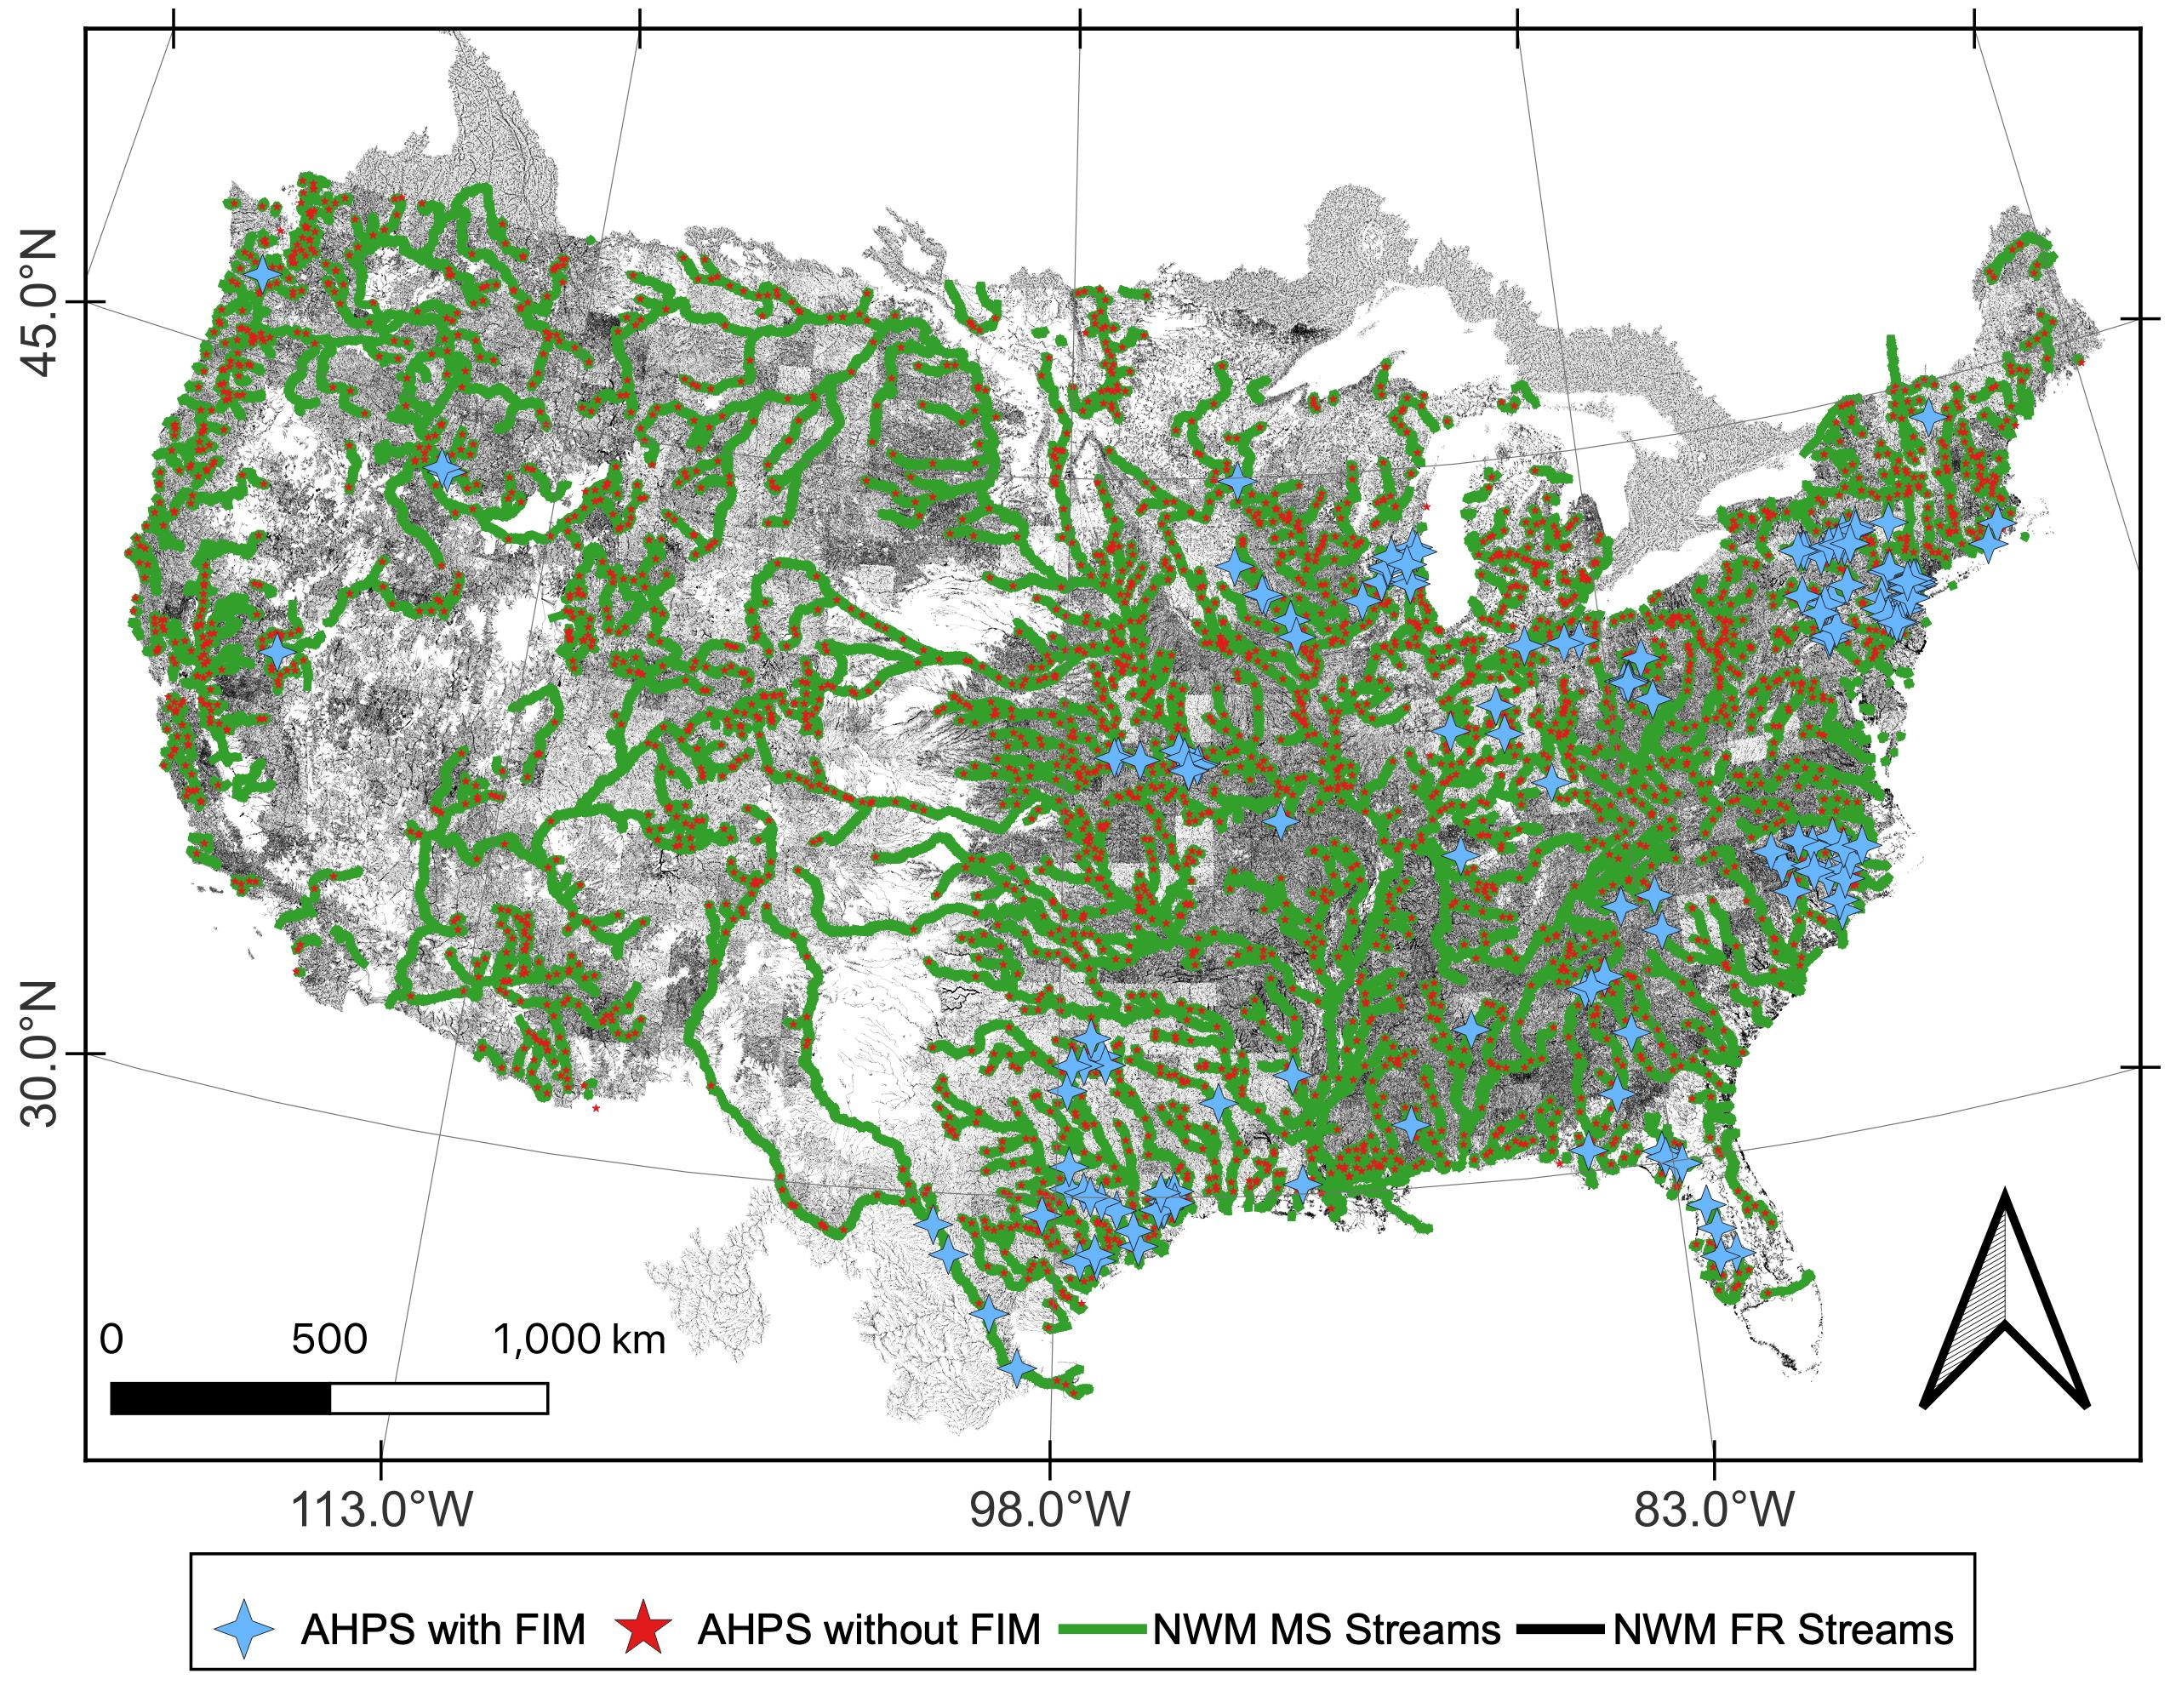
\includegraphics[scale=1.0]{figures/forecast_points.jpg}
\caption{Forecast points with and without Flood Inundation Maps (FIM) in United States' Advanced Hydrologic Prediction System (AHPS).
Note that only a small fraction of the AHPS forecast points have existing FIM.
Also shown are the National Water Model (NWM) stream networks at the Full Resolution (FR) and Mainstems (MS) resolution.
The FR network constitutes the entire NWM stream network while the MS resolution network is the FR network at or downstream of the AHPS forecast points shown.
}
\label{fig:forecast_points}
\end{figure}
%
%%%%%%%%%%%%%%%%%%%%%%%%%%%%%%%%%%%%%%%%%%%%%%%%%%%%%%%%
\subsection{National Water Model}
\label{ssec:national_water_model}
%%%%%%%%%%%%%%%%%%%%%%%%%%%%%%%%%%%%%%%%%%%%%%%%%%%%%%%%
%
Additional work is required to address the gaps that the AHPS leaves in terms of spatial resolution, spatial coverage, and temporal forecast horizons.
In response to growing stakeholder demand for enhanced and integrated water resource forecasts, the Office of Water Prediction (OWP) at the National Water Center (NWC) along with its partners at the National Center for Atmospheric Research (NCAR) have developed and implemented operationally the NWM which is a configuration of the Weather Research and Forecasting Hydrologic Model (WRF-Hydro) \cite{salas2018towards,gochis2018wrf,cosgrove2019evolution}. 
The NWM forecasts river discharges at more than 2.7 million forecast points at a variety of time horizons including lookback-range (3-28 hrs), short-range (18 hr), medium-range (10 day) and long-range (30 day) forecast horizons.
The NWM enhances the spatial and temporal domain of the current AHPS capabilities operated at the 13 River Forecast Centers (RFC) in areas known as `hydro-blind'.
As a complement to the operational NWM, RFC forecasts from AHPS forecast points are assimilated in the NWM and routed downstream to the next downstream AHPS forecast point where the process iterates again.
This assimilation into NWM is used to enhance forecasting skill by leveraging best available regional-scale forecasts.
The river network upon which this special assimilation technique operates on is herein referred to as the Mainstem (MS) stream network.
Figure \ref{fig:forecast_points} shows the NWM V2.1 FR stream network as well as the NWM V2.1 MS network.
The MS network contains roughly 120 thousand forecasting points or roughly 4.4\% of the reaches of the FR stream network.

The National Hydrography Dataset Plus (NHDPlus) V2.1 is the basis for the ``hydrofabric'' in the NWM due to its comprehensive use with the hydrologic communities' stakeholders \cite{mckay2012nhdplus,nhdplus2022vectors}. 
The term ``hydrofabric'' is used within the NWM jargon to describe the subset of hydrography composed of the geospatial datasets required for hydrologic modeling including but not limited to stream networks, catchments, channel properties, and elevation data. 
The NWM provides stream forecasts at these hydrofabric segments using the Muskingum-Cunge method to reduce computational requirements of a continental scale model but fails to consider backwater dynamics \cite{bedient2008hydrology,ponce1994variable,gochis2018wrf}.
The need for high-resolution FIM at 10 m or better requires additional post-processing from the principal output of the NWM which is forecast river discharges at the reach scale.
The use of a 2-dimensional (2D) hydrodynamic model across a continental-scale and high spatial resolutions is very cost prohibitive especially in an operational setting.
The Height Above Nearest Drainage (HAND) terrain model is one such technique that can be used, along with synthetic rating curves (SRC), to convert 1-dimensional (1D) riverine discharges to stages, and finally to inundation extents and depths.
%
%%%%%%%%%%%%%%%%%%%%%%%%%%%%%%%%%%%%%%%%%%%%%%%%%%%%%%%%
\subsection{Height Above Nearest Drainage}
%%%%%%%%%%%%%%%%%%%%%%%%%%%%%%%%%%%%%%%%%%%%%%%%%%%%%%%%
%
HAND normalizes topography along the nearest drainage path and it has been demonstrated to be a good proxy and indicator of a series of important environmental conditions including soil environments, landscape classes, soil gravitational potentials, geomorphologies, soil moisture, and groundwater dynamics \cite{renno2008hand,nobre2011height}. 
\citeA{nobre2016hand} showed evidence for utilizing the drainage normalizing HAND dataset as a proxy for flood potential to make static flood inundation maps from known stages.
However, a core assumption made for HAND based FIM is enforcing drainage across the entire area of interest which requires significant digital elevation maps (DEM) manipulations to make a reality.
The terrain index also provides additional utility in the observation of riverine flood inundation mapping from remote sensing especially in areas of high electromagnetic interference such as vegetated and anthropogenic areas \cite{aristizabal2020high,shastry2019using,huang2017comparison,twele2016sentinel}.
\citeA{zheng2018river} developed a methodology for determining stage-discharge relationships known as SRCs by sampling reach-averaged parameters from HAND datasets and inputting into the Manning's equation \cite{gauckler1867etudes,manning1890flow}.
This collection of methods, coupling HAND with SRCs, have been experimented with and compared to other sources of FIM including engineering scale models, in-situ observation, and remote sensing based observation with solid results in large spatial scale applications \cite{godbout2019error,johnson2019integrated,garousi2019terrain,nobre2016hand,afshari2018comparison,zheng2018geoflood,teng2015rapid,teng2017flood,zhang2018comparative}.
%
%%%%%%%%%%%%%%%%%%%%%%%%%%%%%%%%%%%%%%%%%%%%%%%%%%%%%%%%
\subsection{HAND's Assumptions and Limitations}
\label{sssec:hand_assumptions_limitations}
%%%%%%%%%%%%%%%%%%%%%%%%%%%%%%%%%%%%%%%%%%%%%%%%%%%%%%%%
%
HAND operates on many underlying assumptions since it can only be used as an inundation proxy or no physics model and thus, not a true hydrodynamic inundation model \cite{nobre2016hand,liu2016cybergis,liu2020height}.
HAND, to our knowledge, has only been applied to natural, inland, and riverine inundation applications thus it is also missing pluvial, coastal, ground water, and dam break components among other possible sources of flooding.
Additionally, in order to flood an area, HAND assumes all areas eligible for inundation must drain to some nearest stream line which is used for catchment allocation and relative elevation calculation \cite{nobre2016hand,nobre2011height,liu2016cybergis,liu2020height,maidment2017conceptual,garousi2019terrain,zheng2018river,zheng2018geoflood,johnson2019integrated,renno2008hand}.
Stream thalweg networks must also collectively drain to a singular outlet point for a given processing region \cite{nobre2016hand,zheng2018geoflood,renno2008hand}.
Since elevations don't naturally do this, they must undergo a long series of hydro-conditioning processes to enforce monotonically decreasing elevations across an entire processing unit along with hydrologically correct directions of flow \cite{nobre2016hand,nobre2011height,liu2016cybergis,liu2020height,donchyts2016global,renno2008hand}.
The level of DEM manipulation required to enforce this assumption can be substantial depending on the region and can be a significant source of error.
The drainage enforcing assumption also interacts with an inability to properly account for fluvial inundation in regions of DEM depressions that lack natural drainage to riverine areas \cite{nobre2016hand,renno2008hand}.

When used for FIM applications, HAND assumes only fluvial inundation sourced from its nearest drainage line is accounted for \cite{nobre2016hand,mcgehee2016modified}.
Catchments are independent of one another for FIM purposes meaning a reaches' stage value is only used to threshold the HAND values within its respective catchment \cite{liu2016cybergis,zheng2018river,zheng2018geoflood}.
This assumption plays to the ``Nearest Drainage'' term in HAND and creates a significant limitation within HAND for FIM applications \cite{zhang2018comparative,mcgehee2016modified,li2020evaluation,nobre2016hand}.
At the junction of high stream order and high flow rivers with lower flow tributaries, there can be a lack of inundation extents exhibited which is known colloquially in the forecasting community as the ``catchment boundary problem''.
The academic community has somewhat referenced this issue before but it has been characterized more as a problem with the stream delineation process that comes from thresholding the drainage accumulation maps \cite{nobre2016hand,li2020evaluation}.
Later in this study, we will re-introduce this problem and demonstrate how we initialize with a stream network (that of the NWM's) and thus avoid having to threshold accumulations to some arbitrary value to define stream networks.
We illustrate how computing HAND independently for stream lines of unit stream order can significantly enhance FIM performance by accounting for multiple sources of fluvial inundation that may exist in certain regions and flow scenarios.
%
%%%%%%%%%%%%%%%%%%%%%%%%%%%%%%%%%%%%%%%%%%%%%%%%%%%%%%%%
\subsection{HAND Implementations}
%%%%%%%%%%%%%%%%%%%%%%%%%%%%%%%%%%%%%%%%%%%%%%%%%%%%%%%%
%
Due to significant advances in high-performance computing (HPC) and large scale high-resolution DEMs such as the 3D Elevation Program (3DEP) seamless at the 1/3 arc-second (approximately 10 m depending on latitude) scale, HAND has been implemented into software for large-scale, continental computation. 
As part of the OWP's Innovators Program and NWC's Summer Institute, the National Flood Interoperability Experiment (NFIE) generated FIM hydrofabric (will be used interchangeably with the datasets produced by HAND) rapidly on a HPC \cite{maidment2017conceptual,liu2016cybergis}. 
NFIE used open-source dependencies including the Terrain Analysis Using Digital Elevation Models (TauDEM) \cite{tarboton2005terrain} and the Geospatial Data Abstraction Library (GDAL) \cite{warmerdam2008geospatial} to compute HAND for the Continental United States (CONUS) at 331 Hydrologic Unit Code (HUC) 6 processing units in 1.34 CPU years.
By allocating 31 nodes at 20 cores per node for a total of 620 available cores to the overall operation, it enabled the production to finish up in 36 hours consuming 3.2TB of peak memory and 5TB of total disk space.
Originally, NFIE utilized the NHD Medium Resolution (MR) to etch or burn flowlines prior to further conditioning but more recent work has advanced this to the more current NHDPlus High Resolution (NHDPlusHR) which better agrees with the 10 m DEM from the NHDPlusHR program \cite{liu2020height}. 
The original NFIE dataset was employed by the NWC as an unofficial demonstration to produce forecast FIM from the NWM for additional guidance in hydro-blind regions.
Further work by \citeA{djokic2019arc}, implemented a series of improvements to HAND including equidistant reaches, updates to use with NHDPlusHR hydrography, and AGREE DEM reconditioning \cite{hellweger1997agree} into an ESRI Arc-Hydro workflow with use in ArcGIS. 
More notably the software added the ability to derive HAND on both the NWM FR and MS stream networks to consider multiple sources of fluvial inundation along high impact rivers of primary forecasting concern.

Related to these efforts, the United States Geological Survey (USGS) has invested in relative elevation HAND-like methods via work in the GIS Flood Tool (GFT) that also uses SRCs with cross-sections for stage-discharge relationships \cite{verdin2016software}.
Additional investment by \citeA{petrochenkov2020pygft} was able to successfully scale this approach by transitioning the method to open-source Python source code (PyGFT) and implementing novel interpolation methods to help address some of the catchment boundary discontinuities discussed more in this paper.
In addition to the domestic work done in the US, some studies have expanded upon HAND to cover global domains at 30 m resolutions \cite{yamazaki2019merit,donchyts2016global}.
%
%%%%%%%%%%%%%%%%%%%%%%%%%%%%%%%%%%%%%%%%%%%%%%%%%%%%%%%%
\subsection{Office of Water Prediction Flood Inundation Mapping}
%%%%%%%%%%%%%%%%%%%%%%%%%%%%%%%%%%%%%%%%%%%%%%%%%%%%%%%%
%
In order to mitigate the ever increasing threat of flooding to life and property, an operational capability is required to extend NWM streamflow forecasts to river stages, inundation extents, and inundation depths.
OWP FIM is introduced here as a continental scale capability that generates these products at high spatial and temporal resolutions.
Here we introduce OWP FIM that utilizes a few of the latest techniques in HAND based FIM oriented for use with the NWM in continental scale operational forecasting settings. 
Within the operational framework of OWP FIM, we introduce research demonstrating how FIM performance skill with HAND can be improved by discretizing stream networks into units of an effective unit Horton-Strahler stream order \cite{horton1945erosional,strahler1952hypsometric,strahler1952hypsometric} for HAND computation contexts.
Previous authors dating back to the first HAND for FIM work by \citeA{nobre2016hand} have noted a sensitivity of mapping skill to the stream accumulation threshold which is closely related to stream density and the maximum Horton-Strahler stream order (or simply stream order) of the processing unit employed \cite{zhang2018comparative,mcgehee2016modified,li2020evaluation}.
Here we demonstrate how reducing a HAND processing unit's stream network to a singular stream order discretized by level paths (LP), can enhance FIM skill by accounting for multiple possible sources of fluvial inundation.
This capability is introduced progressively as MS (whose network represents about 4\% of FR network) and to a higher degree Generalized Mainstems (GMS) (covers entire FR network) which will be explained later on.
The following methods and results describe the work in more detail and demonstrate its efficacy in producing enhanced FIM for the NWM with applications.
%
